\documentclass[10pt,twocolumn,letterpaper]{article}

\usepackage{iccp}
\usepackage{times}
\usepackage{graphicx}
\graphicspath{{./images/}}
\usepackage{epstopdf}
\usepackage{caption}
\usepackage{subcaption}
\usepackage{amsmath}
\usepackage{amssymb}
\usepackage{url}
\usepackage{bm}
\usepackage{enumerate}

%
% Some new commands I use in this text
%
\newcommand{\OpSphere}{\bm{\mathcal{S}}}
\newcommand{\OpRot}{\bm{\mathcal{R}}}
\newcommand{\OpDistance}{\bm{\mathcal{D}}}
\newcommand{\OpCumsum}{\bm{\mathcal{C}}}
\newcommand{\OpInt}{\bm{\mathcal{I}}}
\newcommand{\OpCamera}{\bm{\mathcal{P}}}
\newcommand{\OpDiag}[1]{\mathrm{diag}\left\{#1\right\}}
\newcommand{\Grad}[1]{\bm{\triangledown_{#1}}}
\newcommand{\argmin}{\mathrm{arg}\min}
\newcommand{\curly}[1]{\left\{#1\right\}}
\newcommand{\roundy}[1]{\left(#1\right)}
\newcommand{\recty}[1]{\left[#1\right]}
\newcommand{\PartDeriv}[2]{\frac{\partial{#1}}{\partial{#2}}}
\newcommand{\vect}[1]{\bm{#1}}
\newcommand{\mat}[1]{\bm{#1}}
\newcommand{\transpose}[1]{{#1}^\intercal}
\newcommand{\derivsym}[1]{\,d{#1}}

%\iccpfinalcopy % *** Uncomment this line for the final submission

\def\iccpPaperID{19} % *** Enter the ICCP Paper ID here
\def\httilde{\mbox{\tt\raisebox{-.5ex}{\symbol{126}}}}

% Pages are numbered in submission mode, and unnumbered in camera-ready
\ificcpfinal\pagestyle{empty}\fi
\begin{document}

%%%%%%%%% TITLE
\title{Sky Tomography for 3D Aerosol Distribution Recovery}

\author{Amit~Aides\\
Electrical Engineering Dept.\\
Technion - Israel Inst. Tech.\\
Haifa 32000, Israel\\
{\tt\small amitibo@tx.technion.ac.il}
\and
Yoav~Y.~Schechner\\
Electrical Engineering Dept.\\
Technion - Israel Inst. Tech.\\
Haifa 32000, Israel\\
{\tt\small yoav@ee.technion.ac.il}
\and
Michael~J.~Garay\\
Jet Propulsion Laboratory\\
California Inst. Tech.\\
CA 91011, United States\\
{\tt\small Michael.J.Garay@jpl.nasa.gov}
%\and
%Vadim~Holodovsky\\
%Electrical Engineering Dept.\\
%Technion - Israel Inst. Tech.\\
%Haifa 32000, Israel\\
%{\tt\small vholod@tx.technion.ac.il}
}

\maketitle
\thispagestyle{empty}

%%%%%%%%% ABSTRACT
\begin{abstract}
  Aerosols, have an important effect on the earth's climate and the
  health of its inhabitants. Nowadays, measurements of atmospheric
  aerosols concentrations is mainly based on spaceborne multi-angular
  hardware as MISR. These methods are usually limited to a layered
  distribution model. We propose a method that has the following
  benefits: it is low cost, and enables 3D recovery of a general
  aerosol distribution over a large area.  To achieve this in a robust
  manner, we use a dense, redundant set of multi-angle images. The
  images are obtained using simple cameras having a wide field of
  view.

  In this work part we first develop an image formation model which
  assumes single-scattering transfer.  Our model enables simulation of
  generally distributed concentrations of aerosols.  We assess the
  validity of the model by also simulating multiple scattering. This
  is done using Monte-Carlo runs.  This reveals the theoretical
  justification and possible limitations to the suggested assumptions.
  Then we show how to use this model to solve the inverse problem:
  given a set of multiangular images, calculate the volumetric aerosol
  distribution.  This is done using optimization methods, exploiting a
  closed-form gradient of a model-fit cost function.
\end{abstract}

%%%%%%%%% BODY TEXT
\section{Introduction}

Lightfield and integral imaging~\cite{bishop,horstmeyer,levoy,kim}  samples the optical radiance distribution in location and direction. So far, this approach has mainly been used in small-scale setups. This paper deals with a huge scale, up to Earth's size.
Notably, the atmosphere we live in allows light to pass through in multiple locations and directions. Light is affected by this medium. Therefore, in this paper we lay out a principle to recover this 3D medium using measured and modeled lightfields. Projecting this large object to various directions is similar to tomography in other scientific domains. However, the formulation is {\em different} than prior situations. Most tomography setups have a controlled and/or multidirectional radiation source~\cite{gorbunov,messer}. In contrast, our source is the uncontrolled, unidirectional Sun. Moreover, typical tomography relies on a linear model~\cite{gregson}: the pixel value is a linear combination of components along a line of sight (LOS), or a multiplicative combination which is linearized by a logarithm. This principle was used to detect a gas in a volcanic plume~\cite{wright}, which absorbs UV. Other gases in the atmosphere absorb IR. However, photographs of the atmosphere are typically dominated by {\em scattering} by particles (aerosols), rather than absorption by gasses. Thus, in contrast to common tomography, in our problem, analysis does not rely on direct illumination, but on sunlight scattered into the LOS. The model turns out to be {\em nonlinear, yet tractable}.

In remote sensing~\cite{diner,kokhan}, imaging through air is associated with {\em atmospheric correction}, based on {\em aerosol retrieval}. In that discipline, the atmosphere is often assumed to be plane-parallel, for simplicity. To meet this assumption, state-of-the-art aerosol retrieval is done in distinct large lateral blocks~\cite{matronchik}, with very limited height resolution~\cite{kalashnikova}. We seek high resolution 3D recovery. Lines of thought from the computational vision and photography community may offer a fresh way to study this medium and the sensing process. In addition to active lightfield descattering~\cite{fuchs,levoy,kim} and recovery of refractive transparent objects~\cite{ihrke}, passive dehazing of ground objects was studied in horizontal, fixed views~\cite{fattal,he,kopf,kratz,narasimhan2,oakley,Hschechner2,tan}. In this paper, however, the medium itself, at all relevant altitudes is the object of interest.

3D recovery of this medium has direct implications to various scientific communities that either rely on remotely-sensed imagery, study the atmosphere, or overcome the medium to see beyond. These include meteorology, atmospheric sciences, volcanology, climatology and planetary sciences. For example, retrieval of aerosols %and clouds
is important for modeling the Earth's radiation transfer, and thus understanding climate factors and evolution~\cite{chud,dayan,kalashnikova}. Aerosol retrieval is also important for monitoring air quality. An example science that focuses of remote observations beyond the medium is oceanic biology: it relies on satellite tracking of chlorophyll distributions~\cite{chang,johnsen,levy,moses}. In such cases, accurate recovery of the atmosphere helps in {\em atmospheric correction}. Beyond Earth, several other bodies in the solar system that have atmospheres (e.g., Sun, Mars, Titan). These objects can be viewed from multiple directions by probes that orbit in solitude, orbit in synchrony with other probes, or flyby. The approach described here may be helpful there.

The results are significant to {\em aviation safety}, which is tightly related to forecasting and real time sensing of the environment around flight
paths. To keep safe, today's coarse sensing limits flight capacity. An extreme example is the 2010 volcanic eruption of Iceland's
Eyjafjallaj$\ddot {\rm o}$kull, whose ash (aerosols) covered much of Europe's airspace, grounding $\approx 100,000$ flights during a week, affecting millions of people. Knowledge of the 3D distribution of the aerosol density might have indicated safe 3D corridors to safely pass through.
The ability to know the conditions in 3D can thus enhance use of flight airspace, while maintaining safety.


This work models passive optical tomographic imaging of the 3D atmospheric scatterer distribution. Then, we solve this tomography problem, to recover the distribution. Recovery is formulated as an optimization that minimizes a cost function. We derive the gradient of this cost function, to enable efficient optimization. Obtaining data for this problem is an interesting task.

Sampling Earth both spatially and angularly is done by the Multiangle Imaging SpectroRadiometer (MISR)~\cite{diner,matronchik} from space (Fig.~\ref{fig:orbit}), the Airborne Multiangle SpectroPolarimetric Imager (AirMSPI)~\cite{dinerDavis07,dinerDavis10}, and other spaceborne and airborne instruments, as POLDER~\cite{baxter,breon,vanMol}. However, the spatial and angular resolution of these instruments is very coarse. We thus believe that high resolution recovery can be achieved if the sky is imaged {\em from below} by large network of ground-based cameras.

%%%%%%%%%%%%%%%%%%%%%%%%%%%%%%%%%%%%%%%%%%%%%%%%%%%%%%%%%%%%%%%%%%%%
%\vspace{-0.25cm}
\section{Theoretical Background}
\label{sec:back}
 \vspace{-0.2cm}

\noindent {\bf Extinction}:
Let sun rays (SR) irradiate a small volume that includes particles of a certain type.
Each particle has a {\em cross section} $\sigma$ (units ${\rm m}^2$)
for interacting with the irradiance (extinction).  The volume includes
many particles of this type. The denser the small volume, the stronger is the extinction.
Let $n$ be the density of the particles (units $1/{\rm m}^3$). Per unit volume, the {\em extinction coefficient} $\beta$ (units $1/{\rm m}$)
is thus given by
\begin{align}
  \beta= \sigma n
  \;.
  \label{eq:extinctc}
\end{align}
Suppose the volume has infinitesimal length $dl$. Then, the relative portion of extinct SR irradiance is
the unitless differential {\em optical depth}
\begin{align}
  d\tau= \beta dl=\sigma n dl
  \;.
  \label{eq:extinct}
\end{align}
If the SR propagates in an extended volume, the optical depth aggregates:
\begin{align}
  \tau= \int d\tau=\int \beta dl=\int \sigma n dl
  \;.
  \label{eq:tau}
\end{align}
Through an attenuating volume, the {\em transmittance} exponentially decays with the optical depth:
\begin{align}
  t=\exp^{-\tau}
  \label{eq:beer-lambert}
\end{align}


\noindent {\bf Scattering}: The interaction (extinction) of a single particle with the irradiance
can be in the form of either absorption or scattering. The weight of scattering (to all directions), relative to the total extinction is given the unitless {\em single scattering albedo} $\varpi$ of the particle.
Per unit volume, the {\em scattering coefficient} $\alpha$ (units $1/{\rm m}$)
is thus given by
\begin{align}
  \alpha= \varpi\beta=\varpi \sigma n
  \;.
  \label{eq:alph}
\end{align}
Scattering is generally anisotropic. The angular distribution of scattering is determined by
a {\em phase function} $P$. Part of the light scatters towards a camera's line of sight (LOS), as illustrated in
Fig.~\ref{fig:settings}. The angle between the SR and LOS is the scattering angle $\Phi^{\rm scatter}$. The phase function
$P(\Phi^{\rm scatter})$ is normalized: its integral over all solid angles is unit. The {\em angular scattering coefficient}
$\tilde\alpha$ has (units $1/({\rm m}\cdot{{\rm strad}}$), and it is given by
\begin{align}
  \tilde\alpha(\Phi^{\rm scatter}) 
  = \varpi\beta P(\Phi^{\rm scatter}) 
  = \varpi \sigma n P(\Phi^{\rm scatter}).
  \label{eq:alphabasic}
\end{align}

The phase function is often approximated by a parametric approximation. A common approximation is the Henyey-Greenstein function,
\begin{align}
  P_g(\Phi^{\rm scatter})\approx
   \frac{3} {8\pi}
   \frac{(1 - g^2)(1+\mu^2)}
        {(2+g^2)(1 + g^2 - 2g\mu)^\frac{3}{2}}
  \label{eq:aerosol_scatter}
\end{align}
where $g$ is the {\em anisotropy parameter} and
\begin{align}
  \mu\equiv \cos \Phi^{\rm scatter}.
   \label{eq:mu}
\end{align}

\noindent {\bf Air molecules}: Molecules are much smaller than the light wavelength $\lambda$. Then, scattering is modeled by the {\em Rayleigh} model: the phase function is
\begin{align}
  P^{\rm air}\left[\mu(k)\right] &= \frac{3}{16\pi}(1+\mu^2)
  \label{eq:rayleighP}
\end{align}
and $\varpi^{\rm air}$=1. Air molecular density $n^{\rm air}$ falls off approximately exponentially with altitude, with a characteristic~\cite{Levi1980} falloff height $H^\mathrm{air}=8\ km$. Consequently~\cite{Levi1980}, the coefficients for extinction and scattering by air molecules are modeled by
\begin{align}
  \alpha^{\rm air}(h, \lambda)=\beta^{\rm air}(h, \lambda)
  \approxeq 1.09 \times 10^{-3}
  \frac{1}{\lambda^4}\exp^{-\frac{h}{H^\mathrm{air}}}.
  \label{eq:rayleighbeta}
\end{align}





%%%%%%%%%%%%%%%%%%%%%%%%%%%%%%%%%%%%%%%%%%%%%%%%%%%%%%%%%%%%%%%%%%%%
%\vspace{-0.25cm}
\section{Forward Model}
\label{sec:skymodel} \vspace{-0.2cm}

Consider Fig.~\ref{fig:groundgrid}. In addition to air molecules, the atmosphere has a non-uniform distribution of scattering aerosols. We seek to recover this 3D volumetric distribution. To solve this problem, we formulate a process analogous to tomographic reconstruction. The scene is projected to multiple directions. Thus, a system captures integrated radiance as a function of direction and 2D projected location. Any voxel in the atmosphere contributes to the integrated radiance in multiple directional measurements. The measurements then provide a large number of constraints, to recover the distribution: the density and type of aerosols, per voxel. In the following, we first describe models for image formation. Then, we describe how the image formation is inverted to recover the 3D sky structure.

Fig.~\ref{fig:groundgrid} shows another possible source for multi-angular imaging through this medium: a set of ground-based wide-angle sky-cameras, looking upwards and capturing the sky lightfield. The location on the surface is ${\bf x}=(x,y)$. Per viewpoint, the view azimuth and elevation angles (relative to the zenith and north) are encapsulated in the vector ${\bf{\Theta}}$.  A raw image is $i_{\bf x}({\bf{\Theta}})$: the ground location is fixed per frame, while any pixel in a frame represents an angle ${\bf{\Theta}}$.

Sunlight is scattered in the medium along the LOS, creating {\em airlight}~\cite{fattal,narasimhan2,Hschechner2,tan}. For each view ${\bf{\Theta}}$ and ground location ${\bf x}$, the airlight is generally different, depending on the distribution of aerosols both along the LOS, and the along the SRs that hit the LOS.
As Fig.~\ref{fig:groundgrid} shows, for different ${\bf x}$ and ${\bf{\Theta}}$, the LOS cuts through a different set of voxels in the atmosphere. Thus, for each view, the radiance scattered from a voxel is attenuated differently, depending on the distribution of aerosols along the LOS~\cite{hansen}.

Given a scene, the measured radiance for all locations ${\bf x}$ and angles ${\bf{\Theta}}$ is a four dimensional {\em lightfield} $I({\bf x},{\bf{\Theta}})$. Individual images are slices of the lightfield. A typical raw image is $i_{\bf x}({\bf{\Theta}})$: the ground location is fixed per frame, while any pixel in a frame represents an angle ${\bf{\Theta}}$.
The cameras may be static in a network of fixed nodes.
 %Alternatively, several ground-based cameras can be mounted on moving vehicles, assuming that the aerosol distribution does not change much during the time-lapse of the camera trajectory.
\begin{figure*}[b!]
   \begin{center}
\vspace{-0.4cm}
    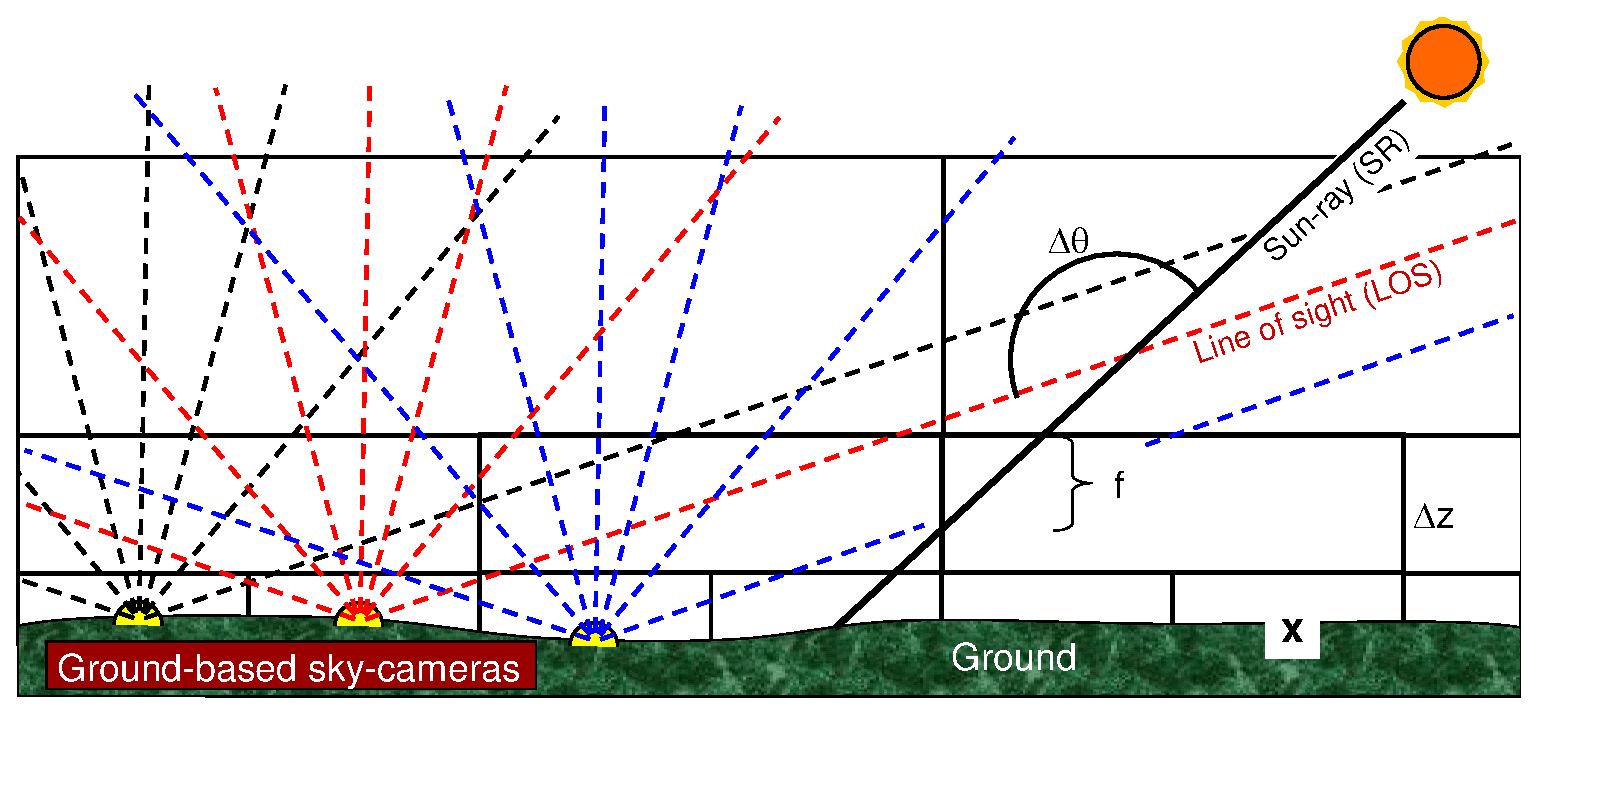
\includegraphics[width=0.99\linewidth]{groundtomog6.eps}
    \end{center}\vspace{-1.5cm}
    \caption{\small
    Lightfield imaging through a volumetric distribution in
    the atmosphere, using ground-based cameras. Our tomographic reconstruction
    follows the acquisition. Irrespective of imaging from space or land, this figure represents the atmosphere in a non-parametric structure, yet the voxel grid gets coarser with altitude, expressing a prior about natural regularity.}
   \label{fig:groundgrid}
\end{figure*}

A forward model calculates the image captured by each camera.
Its input is the aerosol distribution, and it calculates radiative
transfer. We use a single scattering model, in which any SR changes direction (scatters)
only once on the way to the camera.
Under single-scattering approximation, this transfer has three steps (Fig.~\ref{fig:settings}):
\begin{enumerate}
\item SR attenuation, as it propagates from the top of the atmosphere
  (TOA) to voxel $k$.
\item Light scattering at voxel $k$, towards a camera.
\item LOS attenuation, as light propagates from voxel $k$ to the camera.
\end{enumerate}
Steps 1 and 3 calculates the optical depth
along the light path to and from voxel $k$. This is described in Sec.~\ref{sec:optical-depth}.
Step 2 calculates the scattering coefficient at voxel $k$,
as described in Sec.~\ref{sec:scattering}.

%The light transfer, $\mathrm{t}(k)$, is calculated per scattering at
%each voxel $k$.  Let the Sun irradiance at the TOA be $\mathrm{L}^{\rm
%  TOA}$.  The overall transmittance multiplied by $\mathrm{L}^{\rm
%  TOA}$ yields the radiance sensed by the camera. The sum of
%contributions from all voxels is the image captured by the camera,
%\begin{align}
%  \mathrm{I}_{\rm camera}=\mathrm{L}^{\rm TOA} \sum_k \mathrm{t}(k).
%  \label{eq:transatsensor}
%\end{align}

\begin{figure}
  \centering \def\svgwidth{0.8\columnwidth}
  \input{images/atmo_settings.pdf_tex}
  \caption[Settings of the atmosphere simulation]{Settings for the
    atmosphere simulation.}
  \label{fig:settings}
\end{figure}




\begin{figure}
  \centering
    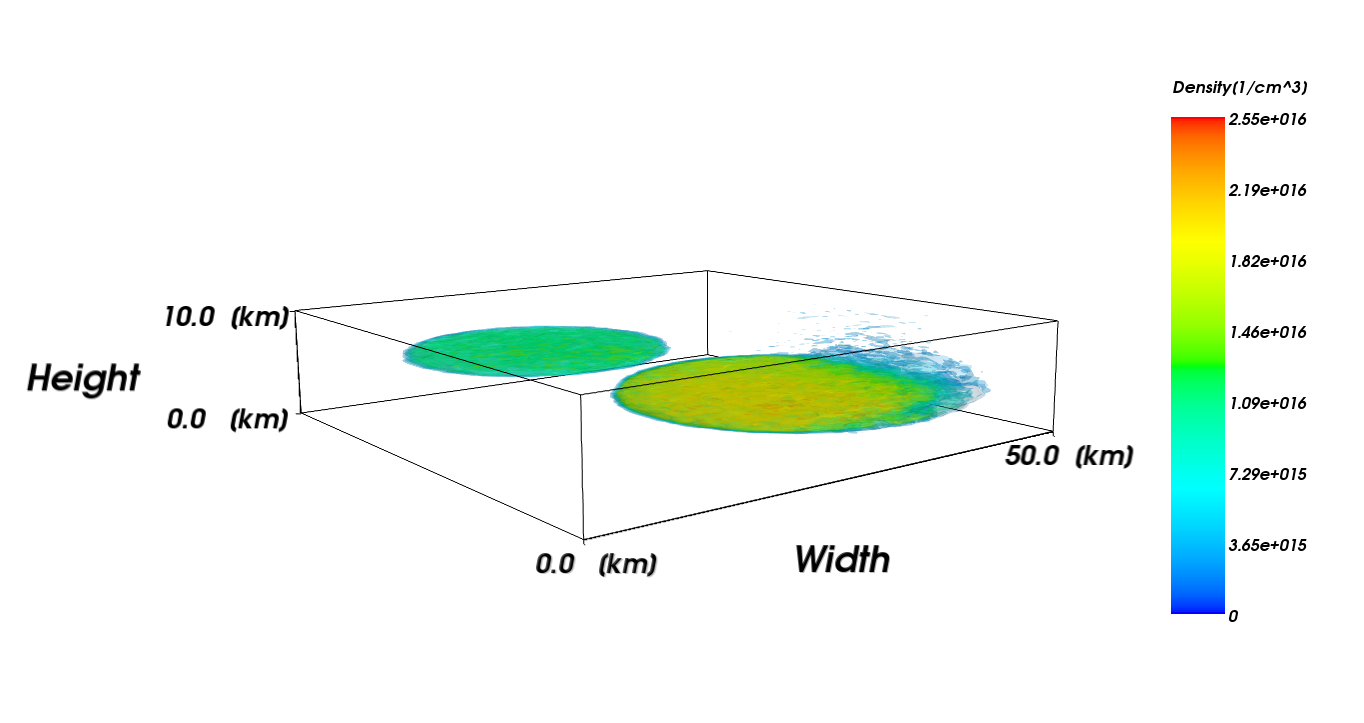
\includegraphics[width=\columnwidth]{images/front.png}
    \caption{Reconstruction of a synthetic aerosol distibution.}
  \label{fig:front}
\end{figure}

%%%%%%%%%%%%%%%%%%%%%%%%%%%%%%%%%%%%%%%%
\subsection{Optical Depth}
\label{sec:optical-depth}

Let an infinitesimal volume contain aerosols. The extinction and scattering coefficients
due to aerosols in this small volume are, respectively
\begin{equation}
  \beta^{\rm aerosol}=\sigma^{\rm aerosol} n^{\rm aerosol}
  \;\;,\;\;
  \alpha^{\rm aerosol}=\varpi^{\rm aerosol} \beta^{\rm aerosol}
  \;.
  \label{eq:betaer}
\end{equation}
In addition, the infinitesimal volume contain also air molecules. Hence, the overall
extinction and scattering coefficients in this small volume are, respectively
\begin{equation}
  \beta=\beta^{\rm air}+\beta^{\rm aerosol}
  \;\;,\;\;
  \alpha=\alpha^{\rm air}+\alpha^{\rm aerosol}
  \;.
  \label{eq:betair}
\end{equation}

Any voxel generally contains both air molecules and aerosols. Voxels are indexed by $k$ or $q$.
As approximation, assume that within any voxel, the molecular parameters
$\{ \beta^{\rm air}(k),\alpha^{\rm air}(k)\}$ and the aerosol parameters
$\{ \sigma^{\rm aerosol}(k),\varpi^{\rm aerosol}(k), n^{\rm aerosol}(k),g(k)\}$
are constants, e.g., corresponding to the value at each voxel center. These parameters generally change
between voxels.

A voxel's vertical geometric thickness is $\Delta z$.  The Sun zenith angle is $\Phi^{\rm SR}$.
Denote a SR line segment between the TOA and the center of voxel $k$ by $[{\rm SR},k]$.
This SR intersects voxel $q$. The geometric length of this intersection
line segment is $\Delta z f_{\rm SR}(q)/\cos\Phi^{\rm SR}$: the factor
$f_{\rm SR}(q)\in [0,1]$ expresses how much of the vertical thickness of $q$ is crossed by the SR.
Following Eq.~(\ref{eq:tau}), the optical depth between the TOA and voxel $k$ is
\begin{equation}
  \tau_{\rm SR}(k)=\frac{1}{\cos\Phi^{\rm SR}}
     \sum_{q \in[{\rm SR},k]}
     \beta(q)\Delta z  f_{\rm SR}(q)
  \;\;.
  \label{eq:lSRn}
\end{equation}
\begin{figure}
  \centering
    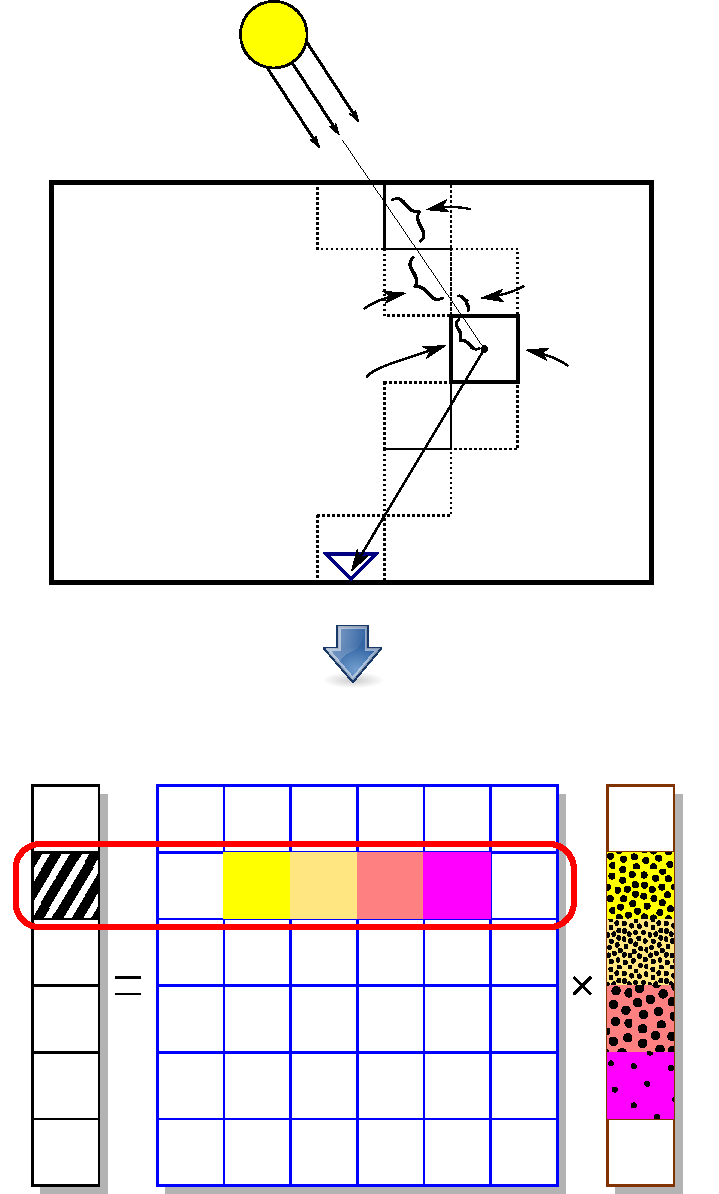
\includegraphics[width=\columnwidth]{images/optical_distance.pdf}
  \caption{Optical depth calculation}
  \label{fig:projection}
\end{figure}
Eq.~(\ref{eq:lSRn}) can be written as
\begin{equation}
  \tau_{\rm SR}(k)=
   \tau_{\rm SR}^{\rm air}(k) +  \tau_{\rm SR}^{\rm aerosol}(k)
  \;\;,
  \label{eq:lSRaa}
\end{equation}
where
\begin{equation}
  \tau_{\rm SR}^{\rm air}=\frac{\Delta z}{\cos\Phi^{\rm SR}}
     \sum_{q \in[{\rm SR},k]}
     \beta^{\rm air}(q)  f_{\rm SR}(q)
  \label{eq:lSRair}
\end{equation}
and
\begin{equation}
  \tau_{\rm SR}^{\rm aerosol}(k)=\frac{\Delta z}{\cos\Phi^{\rm SR}}
     \sum_{q \in[{\rm SR},k]}
     \sigma^{\rm aerosol}(q) n^{\rm aerosol}(q) f_{\rm SR}(q)
  \label{eq:lSRaeros}
\end{equation}


We concatenate all voxels into a columns stack vector. Thus 
aerosol densities and cross sections in all voxels are stored in the respective vectors
${\bf n}$ and $\vect{\sigma}$.
Eq.~(\ref{eq:lSRaeros}) leads to a vector of SR optical depths due to aerosols:
\begin{equation}
  \vect{\tau}_{\rm SR}^{\rm aerosol}=
  {\bf D}^{\mathrm{Sun \rightarrow voxel}}
     (\vect{\sigma} \odot {\bf n})
  \label{eq:tauSRvec1}
\end{equation}
where the operator $\odot$ denotes the Hadamard (element-wise)
product. The non-zero elements of the sparse matrix ${\bf D}^{\mathrm{Sun \rightarrow voxel}}$
represent $[\Delta z/\cos\Phi^{\rm SR}]f_{\rm SR}(q)$, \mbox{$\forall q \in[{\rm SR},k],$} $\forall k$.
Similarly, Eq.~(\ref{eq:lSRair}) leads to a vector of SR optical depths due to air,
$\vect{\tau}_{\rm SR}^{\rm air}$.


Analogously, for camera $c$, denote by $[{\rm LOS}_c,k]$
a LOS bounded between the camera and the center of voxel $k$. The LOS zenith angle is $\Phi^{\rm LOS}_c$.
This LOS intersects voxel $q$. The geometric length of this intersection
line segment is $\Delta z f_{\rm LOS_c}(q)/\cos\Phi^{\rm LOS}_c$: the factor
$f_{\rm LOS_c}(q)\in [0,1]$ expresses how much of the vertical thickness of $q$ is crossed by the LOS.
Following Eq.~(\ref{eq:tau}), the optical depth between the TOA and voxel $k$ is
Analogously to Eqs.~(\ref{eq:lSRaa},\ref{eq:lSRair},\ref{eq:lSRaeros}),
The optical depth %path length
along a LOS to $k$ is
\begin{equation}
  \tau_{{\rm LOS}_c}(k)=
   \tau_{{\rm LOS}_c}^{\rm air}(k) +  \tau_{{\rm LOS}_c}^{\rm aerosol}(k)
  \;\;,
  \label{eq:lLOSaero}
\end{equation}
where
\begin{equation}
  \tau_{{\rm LOS}_c}^{\rm air}(k)=\frac{\Delta z}{\cos\Phi^{\rm LOS}_c}
     \sum_{q \in[{\rm LOS}_c,k]}
     \beta^{\rm air}(q)  f_{\rm LOS_c}(q)
  \label{eq:lLOSaero}
\end{equation}
and
\begin{align}
  \tau_{{\rm LOS}_c}^{\rm aerosol}(k)=
  ~~~~~~~~~~~~~~~~~~~~~~~~~~~~~~~~~~~~~
  ~~~~~~~~~~~~~~~~~~%\nonumber
  ~~~~~
  \\
  %~~~~ 
   \frac{\Delta z}{\cos\Phi^{\rm LOS}_c}
     \sum_{q \in[{\rm LOS}_c,k]}
     \sigma^{\rm aerosol}(q) n^{\rm aerosol}(q) f_{\rm LOS_c}(q)
     \nonumber 
  \label{eq:lLOSaeros}
\end{align}
Eq.~(\ref{eq:lLOSaeros}) leads to a vector of LOS optical depths due to aerosols:
\begin{equation}
  \vect{\tau}_{{\rm LOS}_c}^{\rm aerosol}=
  {\bf D}^{\mathrm{voxel \rightarrow cam}}_c
     (\vect{\sigma} \odot {\bf n})
  \label{eq:tauLOSvec1}
\end{equation}
The non-zero elements of the sparse matrix ${\bf D}^{\mathrm{voxel \rightarrow cam}}_c$
represent $[\Delta z/\cos\Phi^{\rm LOS}_c]f_{\rm LOS_c}(q)$,
\mbox{$\forall q \in[{\rm LOS}_c,k],$} $\forall k$.
Similarly, Eq.~(\ref{eq:lSRair}) leads to a vector of LOS optical depths due to air,
$\vect{\tau}_{{\rm LOS}_c}^{\rm air}$.

The fixed sparse matrices ${\bf D}^{\mathrm{Sun \rightarrow voxel}}$ and
${\bf D}^{\mathrm{voxel \rightarrow cam}}_c$ are compounded to a single matrix
\begin{equation}
  {\bf D}_c=
  {\bf D}^{\mathrm{Sun \rightarrow voxel}}+
  {\bf D}^{\mathrm{voxel \rightarrow cam}}_c
  \;\;.
  \label{eq:Dtotal}
\end{equation}
Similarly, the molecular optical depths along all trajectories between the sun, each voxel
and camera $c$ is compounded to a vector
\begin{equation}
  \vect{\tau}_c^{\rm air}=
  \vect{\tau}_{\rm SR}^{\rm air}+
  \vect{\tau}_{{\rm LOS}_c}^{\rm air}
  \;\;.
  \label{eq:tauairtotal}
\end{equation}
Using Eq.~(\ref{eq:rayleighbeta}) for $\beta^{\rm air}$ in all voxels,
the vector $\vect{\tau}_c^{\rm air}$ is fixed. Thus $\vect{\tau}_c^{\rm air}$ can
be calculated once, per sun zenith angle.

Using Eqs.~(\ref{eq:lSRaa},\ref{eq:tauSRvec1},\ref{eq:lLOSaero},\ref{eq:tauLOSvec1},\ref{eq:Dtotal},\ref{eq:tauairtotal}),
The total optical depths corresponding to SRs and LOSs (of camera $c$) that cross all voxels comprise the vector
\begin{equation}
  \vect{\tau}_c= \vect{\tau}_c^{\rm air}
               + {\bf D}_c (\vect{\sigma} \odot {\bf n})
  \;\;.
  \label{eq:tautotal}
\end{equation}
This vector depends on the variables $\vect{\sigma}$ and ${\bf n}$.

%%%%%%%%%%%%%%%%%%%%%%%%%%%%%%%%%%%%%%%
\subsection{Scattering}
\label{sec:scattering}

Per camera $c$ and voxel $k$, the lines $[{\rm SR},k]$ and $[{\rm LOS}_c,k]$ intersect at a
fixed angle $\Phi^{\rm scatter}_c(k)$, which is pre-calculated.
%Eq.~(\ref{eq:mu})  yields its cosine, $\mu_c(k)$.
Column-stacking all voxels yields the vector representation of all scattering angles in the domain, $\vect{\Phi}^{\rm scatter}_c$ per camera $c$. Similarly, the single-scattering albdeos
$\varpi^{\rm aerosol}$ in all voxels are stacked to vector $\vect{\varpi}$.
Using Eqs.~(\ref{eq:alphabasic},\ref{eq:rayleighP},\ref{eq:betaer},\ref{eq:betair}), the angular scattering coefficients across the domain are expressed in vector form by
\begin{align}
  \tilde{\vect{\alpha}}^{\rm air}_c &=
    \vect{\beta}^{\rm air} \odot P^{\rm air}(\vect{\Phi}^{\rm scatter}_c)   \nonumber \\
  \tilde{\vect{\alpha}}^{\rm aerosol}_c &=
     \vect{\varpi}\odot
     \vect{\sigma} \odot
     {\bf n} \odot
     P^{\rm aerosol}_{\bf g}(\vect{\Phi}^{\rm scatter}_c)
  \label{eq:alpha_matrix}
\end{align}
The vector ${\bf g}$ column-stacks the anisotropy parameter of the phase function, in all voxels. We use this notation, to use a parametric phase function as in Eq.~(\ref{eq:aerosol_scatter}).


%%%%%%%%%%%%%%%%%%%%%%%%%%%%%%%%%%%%%%%%%%%%%%%%%%%%%%%%%%%%%%%%
\subsection{Image Capture}
\label{sec:captured-image}

Compounding the attenuation of irradiance along both $[{\rm SR},k]$ and $[{\rm LOS}_c,k]$, and scattering
by voxel $k$ towards the camera (Eqs.~\ref{eq:beer-lambert},\ref{eq:betair},\ref{eq:tautotal}), the radiant power contributed by the voxel is
\begin{equation}
  p_c(k)= L^{\rm TOA}
          [\tilde{\alpha}^{\rm air}_c(k) + \tilde{\alpha}^{\rm aerosol}_c(k)]
          e^{-[\tau_c(k)]}
  \;\;.
  \label{eq:ick}
\end{equation}
A column-stack vector of all voxel contributions is
\begin{equation}
 {\bf p}_c= L^{\rm TOA}
          [\tilde{\vect{\alpha}}^{\rm air}_c + \tilde{\vect{\alpha}}^{\rm aerosol}_c]
           \odot e^{-\vect{\tau}_c}
  \;\;.
  \label{eq:pc}
\end{equation}
A camera pixel collects light from a narrow cone in the atmosphere.
The cone includes some voxels, intersects with some other voxels, and oblivious to all the rest.
\begin{figure}
  \centering
    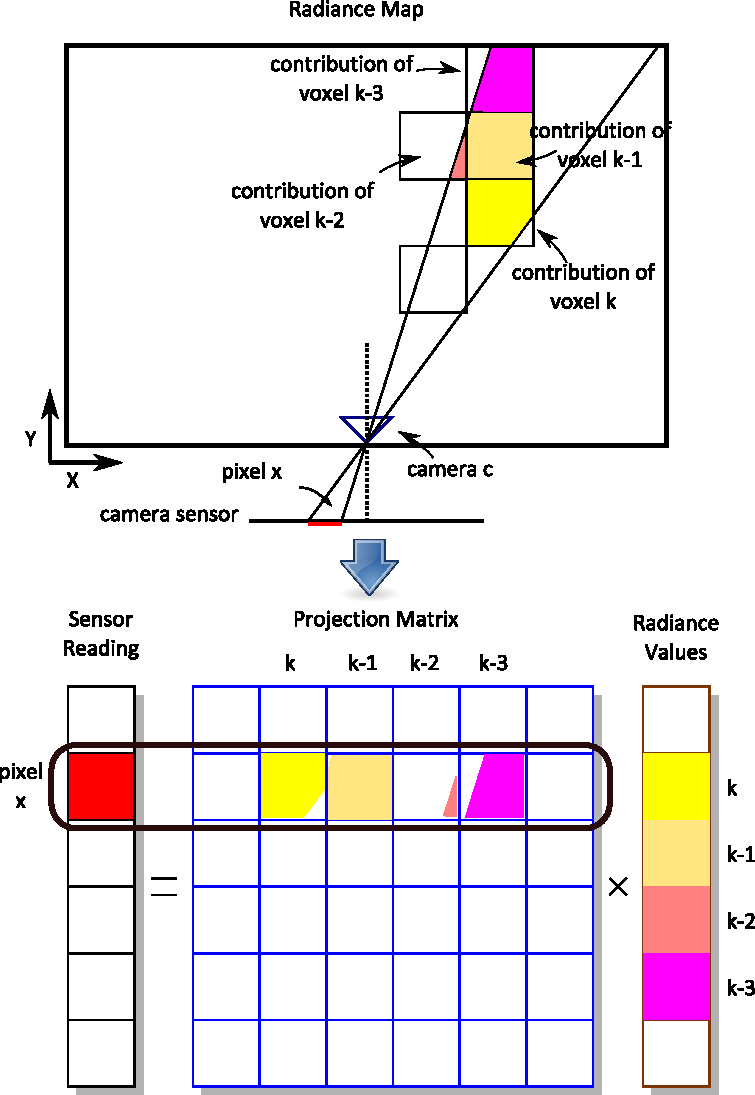
\includegraphics[width=\columnwidth]{images/sensor.pdf}
  \caption{Camera projection operation}
  \label{fig:projection}
\end{figure}
Thus the measured radiance at a pixel is weighted sum of the power $p_c(k)$ from all voxels: most voxels have null weight, since they fall outside the pixels's conic field of view, while the rest of the voxels are aggregated.

This linear sum is formulated by a matrix operation over ${\bf p}_c$. The measured radiance is
\begin{equation}
 {\bf I}_c= {\vect{\Pi}}_c{\bf p}_c
  \;\;,
  \label{eq:IcP}
\end{equation}
where the sparse ${\vect{\Pi}}_c$ matrix expresses {\em projection} of light into camera $c$.
For pixel $\Theta$ and voxel $k$, there is an {\em intersection} volume ${\bf V}_c(\Theta,k)$ between the cone volume of the pixel's field of view, and the voxel, as illustrated in Fig.~\ref{fig:projection}. The corresponding element in the matrix ${\vect{\Pi}}_c$ can be written as
\begin{equation}
 \Pi_c(\Theta,k)=({\rm NA})^2
     \iiint_{{\bf V}_c(\Theta,k)}
     \frac{1}{R({\bf v})^2} d{\bf v}
  \;\;,
  \label{eq:Pc}
\end{equation}
where ${\rm NA}$ is the numerical aperture of the camera lens. The distance $R({\bf v})$ is measured between the camera and an infinitesimal volume element at ${\bf v}\in {\bf V}_c(\Theta,k)$.

Combining Eqs.~(\ref{eq:tautotal},\ref{eq:pc},\ref{eq:IcP}), the captured image is thus
\begin{align}
 {\bf I}_c= L^{\rm TOA}
%  \;\;\;\;\;\;\;\;\;\;\;\;\;\;\;\;\;\;\;\;\;
%  \;\;\;\;\;\;\;\;\;\;\;\;\;
%  ~~~~~~~~~~~~~~~~~~~~~~~~~~~~~~~~~~~~~~
%   \nonumber \\ %\nonumber
%    \cdot
    {\vect{\Pi}}_c
          \left\{
          (\tilde{\vect{\alpha}}^{\rm air}_c + \tilde{\vect{\alpha}}^{\rm aerosol}_c)
           \odot
%           e^{-\vect{\tau}_c}
            e^{-[\vect{\tau}_c^{\rm air}
               + {\bf D}_c (\vect{\sigma} \odot {\bf n})]}
           \right\}
  \label{eq:bigIc}
\end{align}
Most often, there is only a single type of aerosol over a scene. Hence, the three-element
vector $[{\sigma}^{\rm aerosol},\varpi^{\rm aerosol},g]$ is uniform across the scene, but the density distribution ${\bf n}$ is variable. Then, Eq.~(\ref{eq:bigIc}) degenerates to
\begin{align}
 {\bf I}_c= L^{\rm TOA}
    {\vect{\Pi}}_c
          \Big\{
            e^{-(\vect{\tau}_c^{\rm air}
                  + {\sigma}^{\rm aerosol} {\bf D}_c {\bf n})
              }\odot
  \;\;\;\;\;\;\;\;\;\;\;\;\;\;\;\;\;\;\;\;\;
     \nonumber \\
           [\tilde{\vect{\alpha}}^{\rm air}_c + %\right.
           \varpi^{\rm aerosol}\sigma^{\rm aerosol} 
           P^{\rm aerosol}_g(\vect{\Phi}^{\rm scatter}_c)
           \odot{\bf n}
           ]
           \Big\}
           .
  \label{eq:bigIA}
\end{align}
%\begin{align}
% {\bf I}_c= L^{\rm TOA}
%    {\vect{\Pi}}_c
%          \Big(
%            \left\{ \exp
%                 \left[-(\vect{\tau}_c^{\rm air}
%                     + {\sigma}^{\rm aerosol} {\bf D}_c {\bf A}^{\rm aerosol})
%                 \right]
%            \right\}
%%  \;\;\;\;\;\;\;\;\;\;\;\;\;\;\;\;\;\;\;\;\;
%     ~~~~~
%      \nonumber \\ ~~~~~~~~~~~~
%         \odot
%           [\tilde{\vect{\alpha}}^{\rm air}_c + %\right.
%           \tilde\sigma^{\rm aerosol} P^{\rm aerosol}_g(\vect{\Phi}^{\rm scatter}_c)
%           \odot{\bf A}^{\rm aerosol}
%           ]
%           \Big)
%           ,
%  \label{eq:bigIA}
%\end{align}



%\subsection{Simulation Results}
%\label{sec:simulation-results}
%
%Figures~\ref{fig:simulation-results1}
%and~\ref{fig:simulation-results2} show simulated images for different
%aerosol distributions and Sun angles.  The aerosol distribution
%follows the expression below,
%\begin{align}
%  \mat{A}^{\rm aerosol}(h) = \frac{1}{\sigma \times \rm{visibility}}
%  \exp^{-\frac{h}{H^\mathrm{aerosol}}},
%\end{align}
%where $H^\mathrm{aerosol}=1.2\ km$ is a typical characteristic
%thickness of the aerosol layer~\cite{Levi1980}. The `visibility'
%parameter is related to the mean free path (MFP) of the aerosol layer
%at sea level,
%\begin{align}
%  \mathrm{visibility} \triangleq \mathrm{MFP^{sea
%      level}}=\frac{1}{\sigma \mat{A}^{\rm aerosol}_{h=0}},
%\end{align}
%where $\sigma$ is the cross section of the aerosol and $\mat{A}^{\rm
%  aerosol}_{h=0}$ its density at sea level.
%
%In these simulations we use a single type of aerosol (``spherical nonabsorbing 0.06'') across the
%atmosphere. The aerosol properties are taken
%from~\cite{Martonchik2009}.



%%%%%%%%%%%%%%%%%%%%%%%%%%%%%%%%%%%%%%%%%%%%%%%%%%%%%%%%%%%
\section{Inverse Problem}
\label{sec:inverse-problem}

%%%%%%%%%%%%%%%%%%%%%%%%%%%%%%%%%%%%%%%%%%%%%%%%%%%%%%%%%%%
\subsection{Unknowns and Prior Knowledge}
\label{sec:prior}

The atmosphere is photographed from $N_{\rm views}$ viewpoints. Each photograph provides
$N_{\rm pix}$ measurements (pixels), including possible color pixel data in $N_{\rm spectral}$ spectral channels. Hence, the data at our disposal comprises $N_{\rm views}N_{\rm pix}$ measurements.
The number of voxels is  $N_{\rm voxels}$.  In general terms, the variables are the set
\begin{equation}
 {\cal V}\equiv
  \left\{
    {\bf n},
     \left\{
       \vect{\varpi}_{\lambda},\vect{\sigma}^{\rm aerosol}_{\lambda},{\bf g}_{\lambda}
      \right\}_{\lambda}
   \right\}
  \;\;,
  \label{eq:calV}
\end{equation}
where $\lambda$ denotes the spectral channel. Thus, the number of unknown variables is in principle
\mbox{$|{\cal V}|=N_{\rm voxels}(1+3N_{\rm spectral})$}.


Prior knowledge reduces the unknowns. Sec.~\ref{sec:captured-image} mentions a prior:
in many cases a single aerosol type dominates a scene. Then, the three-element
vector $[\varpi,{\sigma}^{\rm aerosol},g]$ is rather spatially uniform. In such cases, the set of unknowns
reduces to
$ {\cal V}=
  \left\{
    {\bf n},
     \left\{
       {\varpi}_{\lambda},{\sigma}^{\rm aerosol}_{\lambda},g_{\lambda}
      \right\}_{\lambda}
   \right\}
$
and \mbox{$|{\cal V}|=N_{\rm voxels}+3N_{\rm spectral}$}.

Furthermore, the elements in the aerosol characteristics
set $\left\{
       {\varpi}_{\lambda},{\sigma}^{\rm aerosol}_{\lambda},g_{\lambda}
      \right\}_{\lambda}$
is not arbitrary, since all these characteristics have physical origins. This
set is constrained to comply with what nature allows (aerosol classes).
This significantly constrains the unknown characteristics. State-of-the-art aerosol retrieval,
as used by NASA's MISR products indeed employ an aerosol-class prior. Types of aerosol mixtures are
discretized to $N_{\rm models}=74$ classes~\cite{martonchikBook}, called {\em models}.
Each class $m$ represents aerosols having a distinct characteristics set.
State of the art retrieval is 1D (only vertical radiative transfer per large areas). We use
this prior in our 3D problem. Then, the set of unknowns reduces to
$ {\cal V}= \left\{ {\bf n},m  \right\}$
and \mbox{$|{\cal V}|=N_{\rm voxels}+N_{\rm models}$}.

%%%%%%%%%%%%%%%%%%%%%%%%%%%%%%%%%%%%%%%%%%%%%%%%%%%%%%%%%%%
\subsection{Objective Function}
\label{sec:objective-function}

The inverse problem (tomography) seeks recovery of the 3D aerosol distribution in the
atmosphere. From Eqs.~(\ref{eq:alpha_matrix},\ref{eq:bigIc},\ref{eq:bigIA},\ref{eq:calV}),
the images $\{ {\bf I}_c\}_{c=1}^{N_{\rm views}}$ depend on the variables set ${\cal V}$, particularly on the unknown field ${\bf n}$. The recovery task is phrased as optimization of a an objective function, that fits the image-formation model~(\ref{eq:bigIc},\ref{eq:bigIA}) to
measured photographs $\{ {\bf I}^{\rm measured}_c\}_{c=1}^{N_{\rm views}}$:
\begin{equation}
  \label{eq:mingenobjective}
  \hat{\cal V} = \argmin_{{\cal V}\in {\cal C}} f({\cal V})
\end{equation}
where
\begin{equation}
  \label{eq:genobjective}
  f({\cal V}) = \sum_{c=1}^{N_{\rm views}}
  \| {\bf I}^{\rm measured}_c - {\bf I}_c({\cal V})\| + {\rm Regularization}({\cal V})
  \;.
\end{equation}
Here ${\cal C}$ is a constraints set, which encapsulates part of the prior knowledge,
as well as nonnegativity bounds, while $\| \|$ is some error-distance measure.
Here term ${\rm Regularization}({\cal V})$ describes spatial regularization terms of the variables, such as smoothness, a blobby or a layered structure.

Spatial regularization can help overcome lack of data, if $N_{\rm views}$ is too small, and it is definitely helpful. In this work, however, we formulate and demonstrate the basic principle of our tomography task, hence
we proceed without regularization. Relying on prior knowledge described in Sec.~\ref{sec:prior}, the problem complexity is by far dominated by the $N_{\rm voxels}$-large array ${\bf n}$, which is continuously valued. Hence, we focus here on retrieving ${\bf n}$ through continuous optimization. Relying on the mean-squared error measure, we seek:
\begin{equation}
  \label{eq:minobjectiveA}
  \hat{\bf n} =
      \argmin_{{\bf n}} f({\bf n})
\end{equation}
where
\begin{equation}
  \label{eq:objectiveA}
  f({\bf n})
   = \sum_{c=1}^{N_{\rm views}}
  \| {\bf I}^{\rm measured}_c - {\bf I}_c({\bf n})\|^2_2
\end{equation}
This is solved using standard optimization tools. Fast optimization that leads to
to local minima ($f$ is not convex) exploits the gradient of $f$. 

Since our model uses close-form expressions, $f$ is differentiable. The gradient of $f$ with respect to ${\bf n}$ is
\begin{align}
  \Grad{\vect{n}} f = -2\sum_{c=1}^{N_{\rm views}}
  \transpose{\left[\mat{J}_{\hat{\vect{i}}_c}(\vect{n})\right]}(\vect{I}_c-\hat{\vect{I}}_c)
  \;.
  \label{eq:gradient1}
\end{align}
Here the matric $\mat{J}_{\hat{\vect{I}}_c}(\vect{a})$ is the Jacobian  of
the vector $\hat{\vect{I}}_c$ with respect to $\vect{n}$. Element $(\Theta,k)$ of this matrix
differentiates the intensity in pixel ${\bf \Theta}$ (in viewpoint $c$) with variation of the density at voxel $k$, i.e.,
  $\partial \hat{\vect{I}}_{c}({\bf \Theta})/\partial{n^{\rm aerosol}(k)}$.
%
%
%
%
%\begin{align}
%  \mat{J}_{\hat{\vect{i}}_c}(\vect{a}) =
%  \begin{pmatrix}
%    \PartDeriv{\hat{\vect{i}}_{c}(1)}{a_1} & \PartDeriv{\hat{\vect{i}}_{c}(2)}{a_2} & \cdots \\
%    \PartDeriv{\hat{\vect{i}}_{c}(1)}{a_1} & \PartDeriv{\hat{\vect{i}}_{c}(2)}{a_2} & \cdots \\
%    \vdots & \vdots & \ddots
%  \end{pmatrix}
%\end{align}

Let $\OpDiag{\vect{\vect{v}}}$ denote conversion of a vector of length
$q$ into a $q \times q$ diagonal matrix,
\begin{equation*}
  \OpDiag{\vect{v}} =
  \begin{bmatrix}
    v_1 & & & \\
    & v_2 & & \text{\huge{0}} \\
    \text{\huge{0}} & & v_3 & \\
    & & & \ddots
  \end{bmatrix}
\end{equation*}

\noindent From~(\ref{eq:atsensor}), we have
\begin{align}
  \mat{J}_{\hat{\vect{i}}_c}(\vect{a}) &= (\rm{NA})^2 \mathrm{L}^{\rm TOA}\,
  \Big( \sigma^{\rm aerosol} \, \varpi \, \OpDiag{P^{\rm
        aerosol}(\vect{\mu}_c)} \transpose{\OpSphere}_c - \nonumber \\
    &\quad \transpose{\OpDistance} \OpDiag{\OpSphere_c (\vect{\alpha}^{\rm
        aerosol}_c +
      \vect{\alpha}^{\rm air}_c )} \Big)
  \OpDiag{\exp^{-(\vect{\tau}^{\rm aerosol}_c + \vect{\tau}^{\rm
        air}_c)}} \transpose{\OpInt} \, \transpose{\OpCamera},
  \label{eq:gradient2}
\end{align}
for detailed derivation of Eq.~(\ref{eq:gradient2}) we refer the
reader to App.~\ref{sec:gradient-derivation}.

%%%%%%%%%%%%%%%%%%%%%%%%%%%%%%%%%%%%%%%%%%%%%%%
\section{Simulations}
\label{sec:simul}

To test the model, we made simulations based on atmospheric models in the literature. Here are the details.\\

\noindent{\bf Sun}: The sun is at zenith angle $\Phi^{\rm SR}=45^o$. Its
$L^{\rm TOA}$ is obtained from~\cite{sun_composition,BBradiance}, with respective red-green-blue rations of
 $L^{\rm TOA}_{\rm R}:L^{\rm TOA}_{\rm G}:L^{\rm TOA}_{\rm B}=255:236:224$.\\

\noindent{\bf Aerosol}: We used particle-type 4 from the aerosol list in
Ref.~\cite{Martonchik2009}. This is a spherical non-absorbing sulfate/sea-sal/organic particle, whose anisotropy parameter per color channel is $[g_{\rm R},g_{\rm G},g_{\rm B}]=[0.718,0.722,0.725]$. Its single-scattering albedo is $\varpi=1$ at all channels. Its extinction cross section per color is
  $[\sigma^{\rm aerosol}_{\rm R},
    \sigma^{\rm aerosol}_{\rm G},
    \sigma^{\rm aerosol}_{\rm B}]=[1.02,1.04,1.03]$.
We set the spatial distribution as a product of two functions. The first function is an exponential decay~\cite{Levi1980} with altitude $h(k)$ of voxel $k$,
\begin{align}
 f_1[h(k)] = \frac{1}
 {\sigma^{\rm aerosol}_{\rm G} \mathrm{MFP^{sea level}}}
  \exp^{-\frac{h(k)}{H^\mathrm{aerosol}}},
\end{align}
where $H^\mathrm{aerosol}=8\ km$. This expresses a general trend of reduced atmospheric density with height. Here
The mean free path (MFP) of the aerosols layer at sea level is
$\mathrm{MFP^{sea level}}=1/50 {\rm[1/km]}$.
% is a typical characteristic thickness of the aerosol layer~\cite{Levi1980}.

The second function, $f_2$, expresses a clustered nature of a aerosol ``clouds''. We define two ellipsoids: the first is centered at altitude
$3.3km$, and has horizontal width of $32km$ and vertical thickness of $2.8km$. The second ellipsoid is centered at altitude $6.6km$, and has lateral width of $24km$ and vertical thickness of $2.1km$. Then
\begin{align}
 f_2(k) = 1 {\rm ~~~if~} k\in {\rm ~any ellipsoid}\\
 f_2(k) = 1 {\rm otherewise},
\end{align}
The aerosol distribution is thus
\begin{align}
  \mat{A}^{\rm aerosol}=f_1(h)f_2.
\end{align}
Note that the horizontal widths are much larger than the vertical ones. This is consistent with scales of atmospheric aerosol distributions.\\

\noindent{\bf Dimensions}: The domain of sky we simulate and recover has area of $50\times 50$km, and it extends from the ground up to altitude of 10km. This volume is divided to a $50\times50\times100$ grid, where each voxel has area of $1\times1$km and vertical thickness of 100 meters. The dimension of the problem is thus ${\cal O}(250,000)$ variables.\\

\noindent{\bf Cameras}: Each ground-based camera has a hemispherical field of view, capturing the entire sky from its viewpoint. We used 95 viewpoints on a grid, each view $\approx 4.4$km from its neighbors.
The resolution of each camera is low: $128\times 128$ pixels, expressing the fact that cloudless (yet hazy) sky images are rather smooth, hence there is no need for high image resolution. Each pixel has full-well depth of 40000 electrons, which corresponds to the brightest pixel value. Each measurement has photon noise, which is Poissonian distributed, according to image value $I_c$ and the full-well depth.\\

\noindent{\bf Computer}: We had access to an SGI-TNN cluster computer that has 88 computer nodes consisting of two 2.40 GHz six-Core Xeon with 8GB
DDR3 memory per core. Out of it, we used 8 nodes, corresponding to 96 cores. Each core was dedicates to render a modeled image (in each interaction) as if captured by a one of the 95 cameras. Each iteration (varying the model according the gradient-based algorithm and varying the all rendered images) took $\approx 7$sec.\\

\noindent{\bf Optimization}: We used a L-BFGS-B algorithm~\cite{BFGS}.
Satisfactory convergence occurred at $\approx 6500$ iterations, taking $\approx 12.5$ hours to complete in total.




\subsection{Optimization Results}
\label{sec:optimization-results}
\begin{figure}
 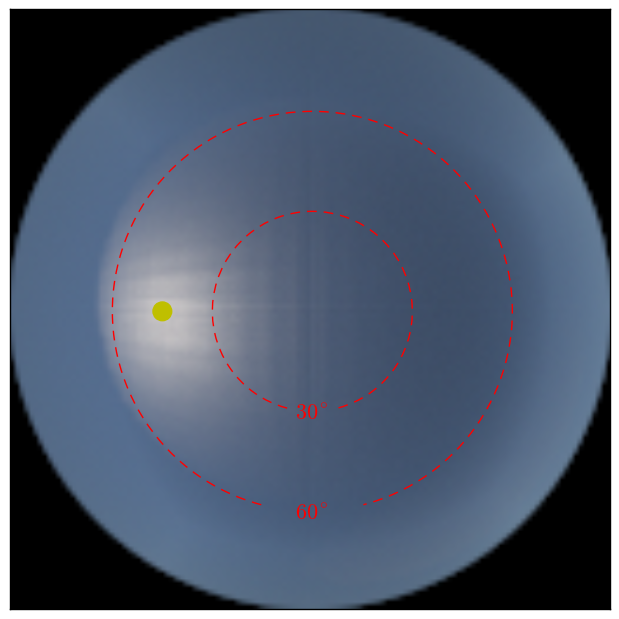
\includegraphics[width=\columnwidth]{images/ref_img34.png}
  \caption{Results of the simulation where the Sun is at top of
    zenith, for different aerosol visibility values. A red dot marks
    the Sun location.}
  \label{fig:simulation-results1}
\end{figure}

\begin{figure}
 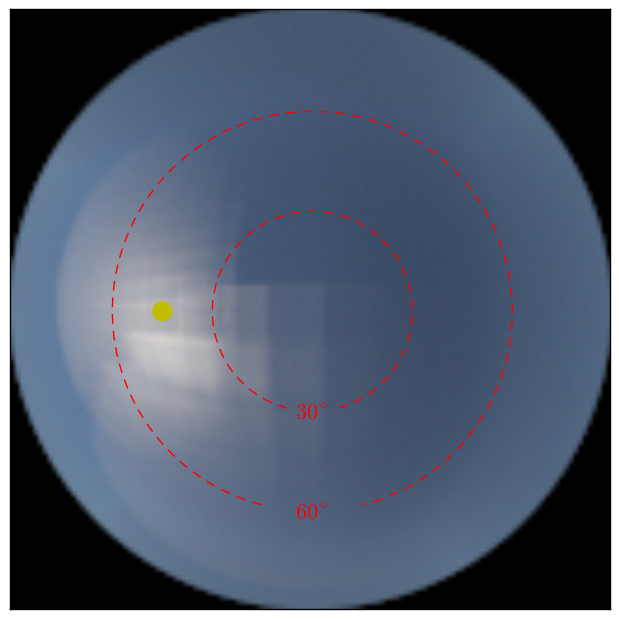
\includegraphics[width=\columnwidth]{images/ref_img37.png}
  \caption{Results of the simulation where the Sun is near the horizon
    for different aerosol visibility values. A red dot marks the Sun
    location.}
  \label{fig:simulation-results2}
\end{figure}


\begin{figure}
  \centering
    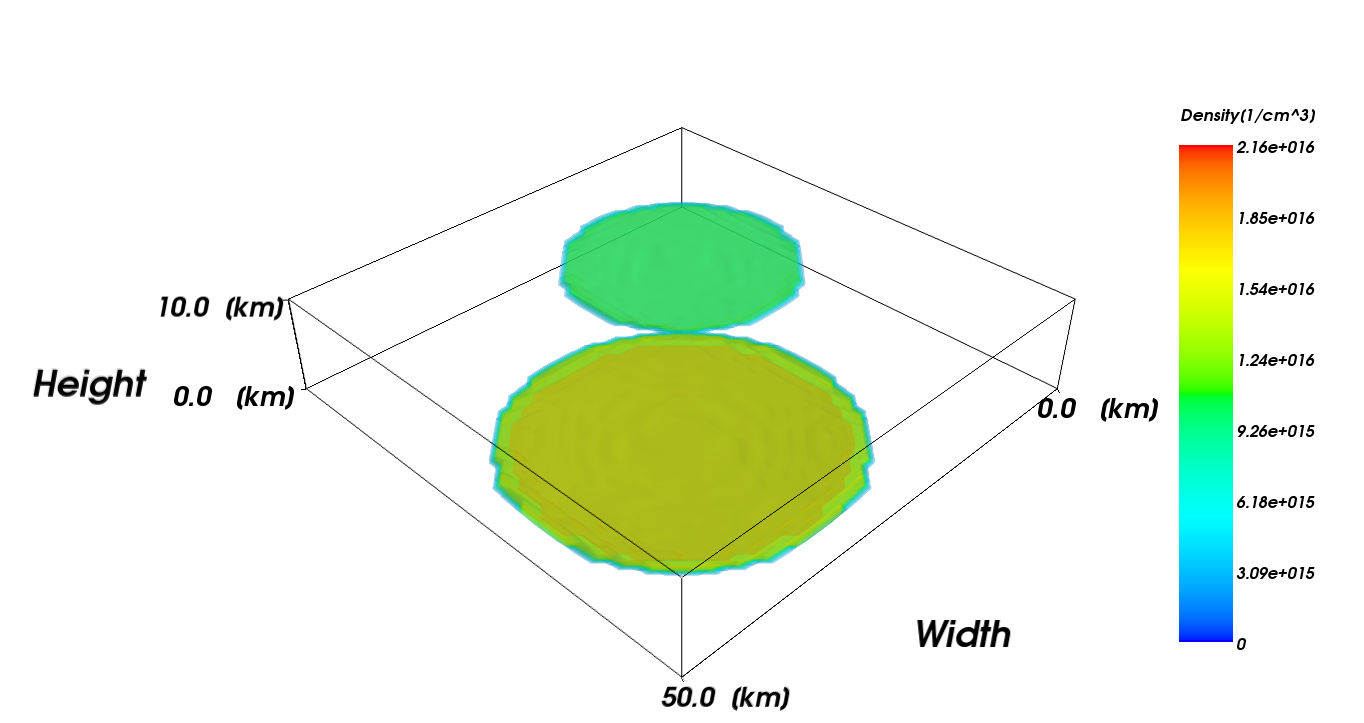
\includegraphics[width=\columnwidth]{images/original}
  \caption{Synthetic 3D aerosol distribution. Colour values mark
    aerosol density.}
  \label{fig:synth-atmo}
\end{figure}

\begin{figure}
  \centering
    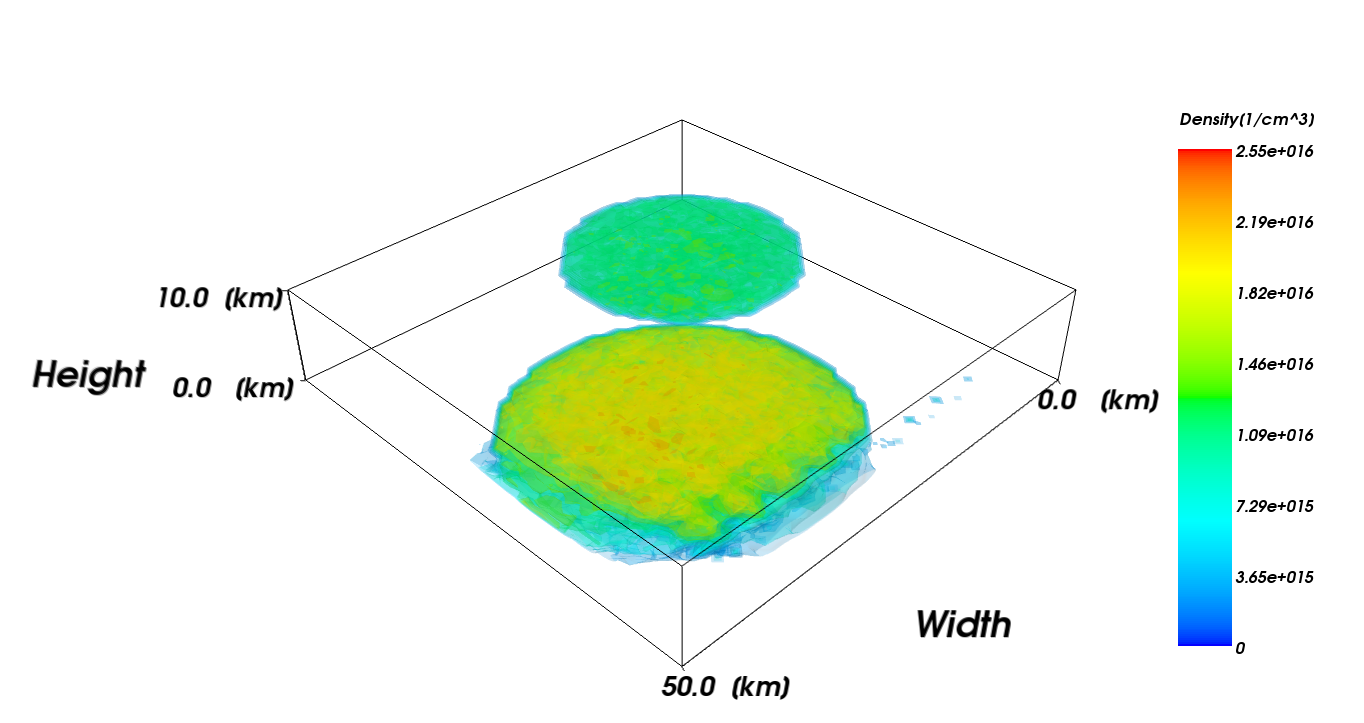
\includegraphics[width=\columnwidth]{images/reconstructed}
  \caption{Reconstructed aerosol distribution.}
  \label{fig:synth-result}
\end{figure}

\appendix

\section{Gradient Derivation}
\label{sec:gradient-derivation}

Here we detail the derivation of~(\ref{eq:gradient2}).  We use
matrices to implement the different operators. Using matrices
simplifies the calculation of derivatives and the use of optimization
tools. Note that~(\ref{eq:atsensor}) in column stack notation is
\begin{align}
  \vect{i}_c=(\rm{NA})^2\mathrm{L}^{\rm TOA} \OpCamera \, \OpInt \,
  \roundy{ \roundy {\OpSphere_c \, \roundy{\vect{\alpha}^{\rm
          aerosol}_c + \vect{\alpha}^{\rm air}_c} } \odot
    \exp^{-(\vect{\tau}^{\rm aerosol}_c + \vect{\tau}^{\rm air}_c)}}.
  \label{eq:atsensor-matrix}
\end{align}
First we show some results relating to differentiation. Let $\vect{a}$
be a vector of length $q$. Let $\vect{g}(\vect{a})$ be a vector
function: it outputs a vector of length $r$. Let $\mat{B}$ be a $q
\times r$ matrix and
\begin{align}
  \vect{g}(\vect{a}) = \exp^{-\transpose{\mat{B}}\vect{a}}.
  \label{eq:example1}
\end{align}
In Eq.~(\ref{eq:example1}), the exponential is element-wise (not
raising an operator to some power). Then
\begin{align}
  \label{eq:partial2}
  \PartDeriv{\vect{g}}{\vect{a}} &= - \mat{B} \,
  \OpDiag{\exp^{-\transpose{\mat{B}}\vect{a}}}
\end{align}
Using~(\ref{eq:partial2}) and~(\ref{eq:tau})
\begin{align}
  \label{eq:partial4}
  \PartDeriv{\exp^{-(\vect{\tau}^{\rm aerosol}_c + \vect{\tau}^{\rm
        air}_c)}}{\vect{a}} &= - \transpose{\OpDistance_c} \,
  \OpDiag{\exp^{-(\vect{\tau}^{\rm aerosol}_c + \vect{\tau}^{\rm
        air}_c)}}
\end{align}

To calculate the derivative of the Hadamard product
in~(\ref{eq:atsensor-matrix}) we first note the following: Let
$\vect{u}(\vect{a})$ be a vector function that outputs a vector of
length $r$. Let $\mat{B}$ be a $r \times q$ matrix. Then,
\begin{align}
  \label{eq:partial1}
  \PartDeriv{\transpose{\mat{B}} (\vect{g} \odot \vect{u})}{\vect{a}}
  = \left[ \PartDeriv{\vect{g}}{\vect{a}} \OpDiag{\vect{u}} +
    \PartDeriv{\vect{u}}{\vect{a}} \OpDiag{\vect{g}} \right]
  \mat{B}.
\end{align}
%
% TODO: Understand if Af \odot Ag = A(f \odot g) and in what terms (on
% A) this is important as in the docs I use the left case and in the
% code I use the right case. It seems to me that it is correct but I
% don't have a proof.
%

Suppose the air distribution is known. Therefore, $\vect{\alpha}^{\rm
  air}_c$ and $\vect{\tau}^{\rm air}_c$ are constant vectors. Then,
\begin{align}
  \label{eq:partial3}
  \PartDeriv{\OpSphere_c \, \vect{\alpha}^{\rm aerosol}_c}{\vect{a}}
  &= \varpi \, \sigma^{\rm aerosol} \, \OpDiag{P^{\rm
      aerosol}(\vect{\mu_c})} \, \transpose{\OpSphere_c}
\end{align}

Based on~(\ref{eq:partial4},~\ref{eq:partial1})
and~(\ref{eq:partial3}) we can calculate the gradient
of~(\ref{eq:atsensor-matrix}):
\begin{align}
  \PartDeriv{\vect{i}_{\rm c}}{\vect{a}} &=
  \mat{J}_{\hat{\vect{i}}_c}(\vect{a})= \nonumber \\
  &= (\rm{NA})^2 \mathrm{L}^{\rm TOA} \, \biggl( \varpi \, \sigma^{\rm
    aerosol} \, \OpDiag{P^{\rm aerosol}(\vect{\mu}_c)} \,
  \transpose{\OpSphere}_c \OpDiag{\exp^{-(\vect{\tau}^{\rm aerosol}_c
      + \vect{\tau}^{\rm
        air}_c)}} \nonumber \\
  &\quad - \transpose{\OpDistance_c} \, \OpDiag{\exp^{-(\vect{\tau}^{\rm
        aerosol}_c + \vect{\tau}^{\rm air}_c)}}\OpDiag{\OpSphere_c \,
    (\vect{\alpha}^{\rm aerosol}_c + \vect{\alpha}^{\rm air}_c)}
  \biggr)
  \, \transpose{\OpInt} \, \transpose{\OpCamera} \nonumber \\
  &= (\rm{NA})^2\mathrm{L}^{\rm TOA} \, \biggl( \sigma^{\rm aerosol}
  \, \varpi \,
  \OpDiag{P^{\rm aerosol}(\vect{\mu}_c)} \, \transpose{\OpSphere_c} - \nonumber \\
  &\quad \transpose{\OpDistance_c} \, \OpDiag{\OpSphere_c \,
    (\vect{\alpha}^{\rm aerosol}_c + \vect{\alpha}^{\rm air}_c )}
  \biggr) \OpDiag{\exp^{-(\vect{\tau}^{\rm aerosol}_c +
      \vect{\tau}^{\rm air}_c)}} \, \transpose{\OpInt} \,
  \transpose{\OpCamera}
\end{align}



{\small
\bibliographystyle{ieee}
\bibliography{atmosphere}
}

\end{document}
